\documentclass[12pt,a4paper, xcolor=table]{article}
\usepackage{graphicx}
\usepackage[utf8]{inputenc}
\usepackage{eurosym}
\usepackage[spanish,es-tabla]{babel}
\usepackage[left=2cm, right=2cm, top=2cm, bottom=2cm]{geometry}
\usepackage{afterpage}
\PassOptionsToPackage{hyphens}{url}\usepackage{hyperref}
\usepackage{subfig}
\usepackage[table,xcdraw]{xcolor}
\usepackage{cite}
\usepackage{url}
\usepackage{changepage}

\usepackage{imakeidx}
\newcommand\blankpage{%
    \null
    \thispagestyle{empty}%
    \addtocounter{page}{-1}%
    \newpage}
\renewcommand*\contentsname{Índice: }

\makeindex
\let\olditemize\itemize
\def\itemize{\olditemize\itemsep=0pt}

\begin{document}
\setlength{\parindent}{0pt}
\begin{titlepage}
        \centering
        
\includegraphics[width=0.75\textwidth]{img/logo_uc3m.jpg}\par\vspace{2cm}
        {\huge\bfseries Práctica Final \\ Predicción del género de libros\par}
        \vspace{0.5cm}
        {\scshape\Large Inteligencia Artificial en las Organizaciones\par}
        \vspace{1.5cm}
        {\scshape\Large Grupo 83-1\par}
        \vspace{1.5cm}
        {\Large\itshape Miguel Gutiérrez Pérez\par}
        {\Large 100383537@alumnos.uc3m.es \par}
        \vspace{1cm}
        {\Large\itshape Mario Lozano Cortés\par}
        {\Large 100383511@alumnos.uc3m.es\par}
        \vspace{1cm}
        {\Large\itshape Alba Reinders Sánchez\par}
        {\Large 100383444@alumnos.uc3m.es\par}
        \vspace{1cm}
        {\Large\itshape Alejandro Valverde Mahou\par}
        {\Large 100383383@alumnos.uc3m.es\par}
        \vspace{5mm}
        {\large GitHub: \textbf{\textit{\href{https://github.com/Pheithar/InteligenciaArtificialOrganizaciones}{InteligenciaArtificialOrganizaciones}}}}
        \vfill

% Bottom of the page
        {\large \today\par}
\end{titlepage}

\tableofcontents

\newpage

\section{Introducción}

El objetivo de esta práctica consiste en abordar una clasificación sobre resúmenes de libros para determinar su género literario. Las razones que llevan a la elección de este problema tienen que ver con que actualmente cualquier persona con la dedicación suficiente puede escribir un libro sin la necesidad del patrocinio de una editorial, lo que conlleva una \textbf{explosión en el número de nuevos libros generados}. Por consiguiente, las librerías y bibliotecas necesitan catalogar una gran cantidad de escritos, lo cual, les lleva a necesitar de métodos de clasificación automática. Por ello, se plantea el uso de resúmenes y meta-datos de los libros puesto que la tarea de clasificación \textbf{debe poder realizarse con el menor número de datos posible}, puesto que no todos los libros que llegan a estas entidades disponen de todos los datos completos.

\vspace{3mm}

La primera cuestión imprescindible que surge al conocer el problema propuesto es qué técnica de Inteligencia Artificial emplear. Dado que se realiza un análisis sobre diferentes textos, la opción evidente es la \textbf{Minería de Texto}, la cual es una técnica de minería de datos que busca extraer \textbf{información útil y relevante de documentos de texto} de diferentes fuentes diferentes, como puede ser páginas web,
correos electrónicos, periódicos o redes sociales. Para ello, se hace una identificación de patrones en los datos, como puede ser la repetición de palabras o conjuntos de palabras, estructuras sintácticas que se repitan a lo largo de los datos, etc. Esta minería de texto tiene numerosas aplicaciones, y en esta práctica se va a desarrollar una clasificación en función de unas categorías que serán definidas gracias a la elección de un conjunto de datos apropiado.

\vspace{3mm}

A continuación se ofrece un \textbf{esquema del funcionamiento de la tarea propuesta} en donde un libro sin catalogación llega a alguna a de estas entidades que necesitan catalogar su género a partir de la información más reducida posible, generalmente título y argumento. Inicialmente se plantea la distinción de un único género, sin embargo, \textbf{es bien sabido que un escrito no tiene por qué adscribirse a un único género} y por lo tanto se debe considerar como futura \textbf{ampliación} catalogar tantos como sea posible.

\vspace{12mm}

  \begin{figure}[!h]
    \centering
    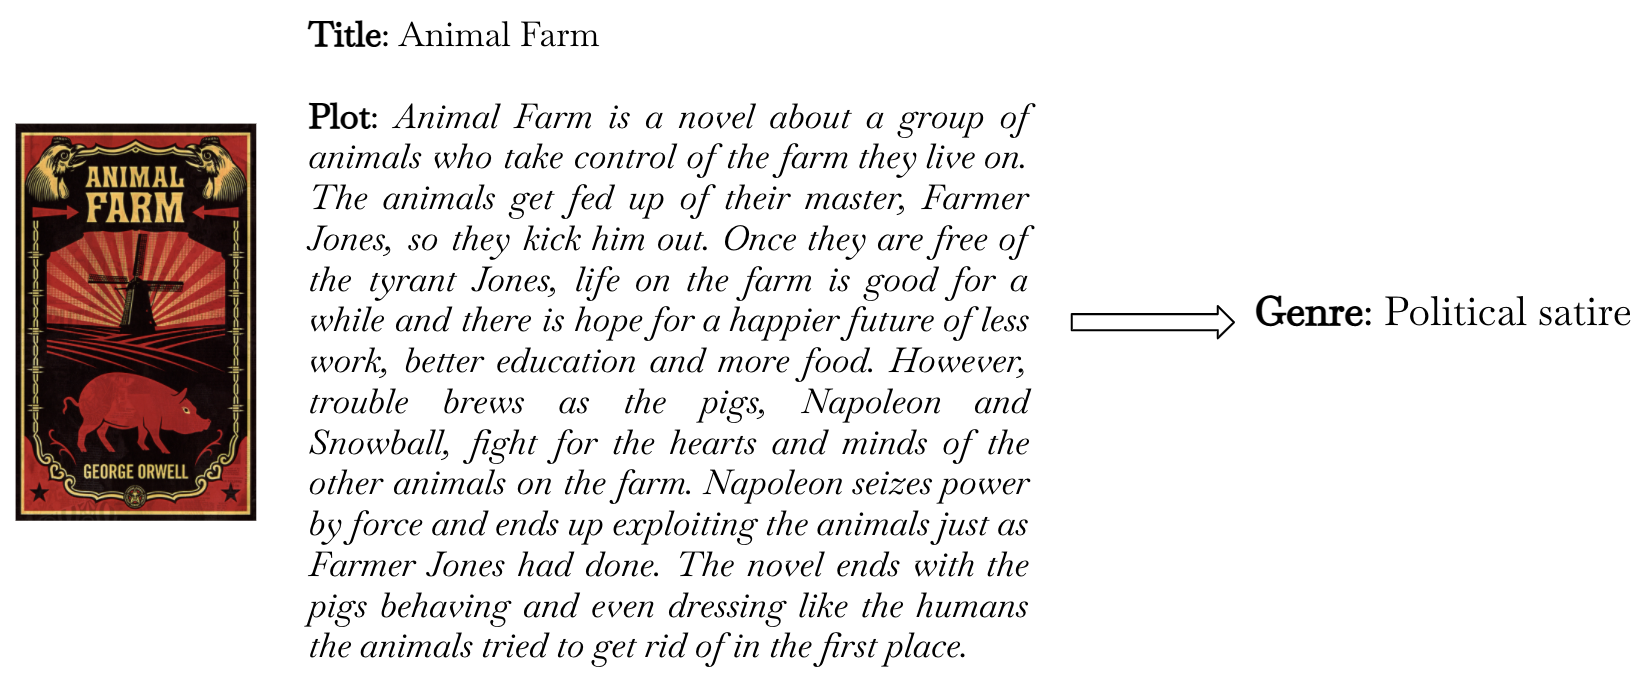
\includegraphics[width=450px]{img/Animal Farm.png}
    \caption{Esquema de la tarea}
    \end{figure}

\newpage

\section{Contexto de la práctica}
La minería de datos, y más en concreto, la Minería de Texto, tal y como se ha comentado en trabajos pasados, es un área que está sufriendo una gran revolución gracias a las redes neuronales. Esta revolución es similar a la que sufrieron las redes convolucionales desde la aparición de las arquitecturas de Deep Learning y permite enfoques novedosos como el desarrollado en esta práctica gracias a la técnica de \textit{embeddings}. 

\vspace{3mm}

La aplicación de \textit{embeddings} supone por lo tanto un punto de partida muy interesante para numerosas tareas de \textit{text-mining}, así, se encuentran \textit{paper} académicos que muestran las ventajas y mejora de resultados obtenidas por estas técnicas. En este contexto surge el estudio de Alex Dekhtyar y Vivian Fong sobre la catalogación de requisitos de software aplicando \textit{embeddings} y comparando los resultados con los obtenidos con otras técnicas como Naïve Bayes [Referencia]. El objetivo de dicho estudio era realizar clasificación sobre requisitos relacionados y no relacionados con asuntos de seguridad. Usando para ello las arquitecturas de\textit{ word embedding }\textit{word2vect desarrolladas} por Google [Referencia] se puede obtener una representación semántica muy acertada de las palabras. La arquitectura propuesta es por lo tanto muy similar a una red neuronal convolucional de procesamiento de imágenes.

  \begin{figure}[!h]
    \centering
    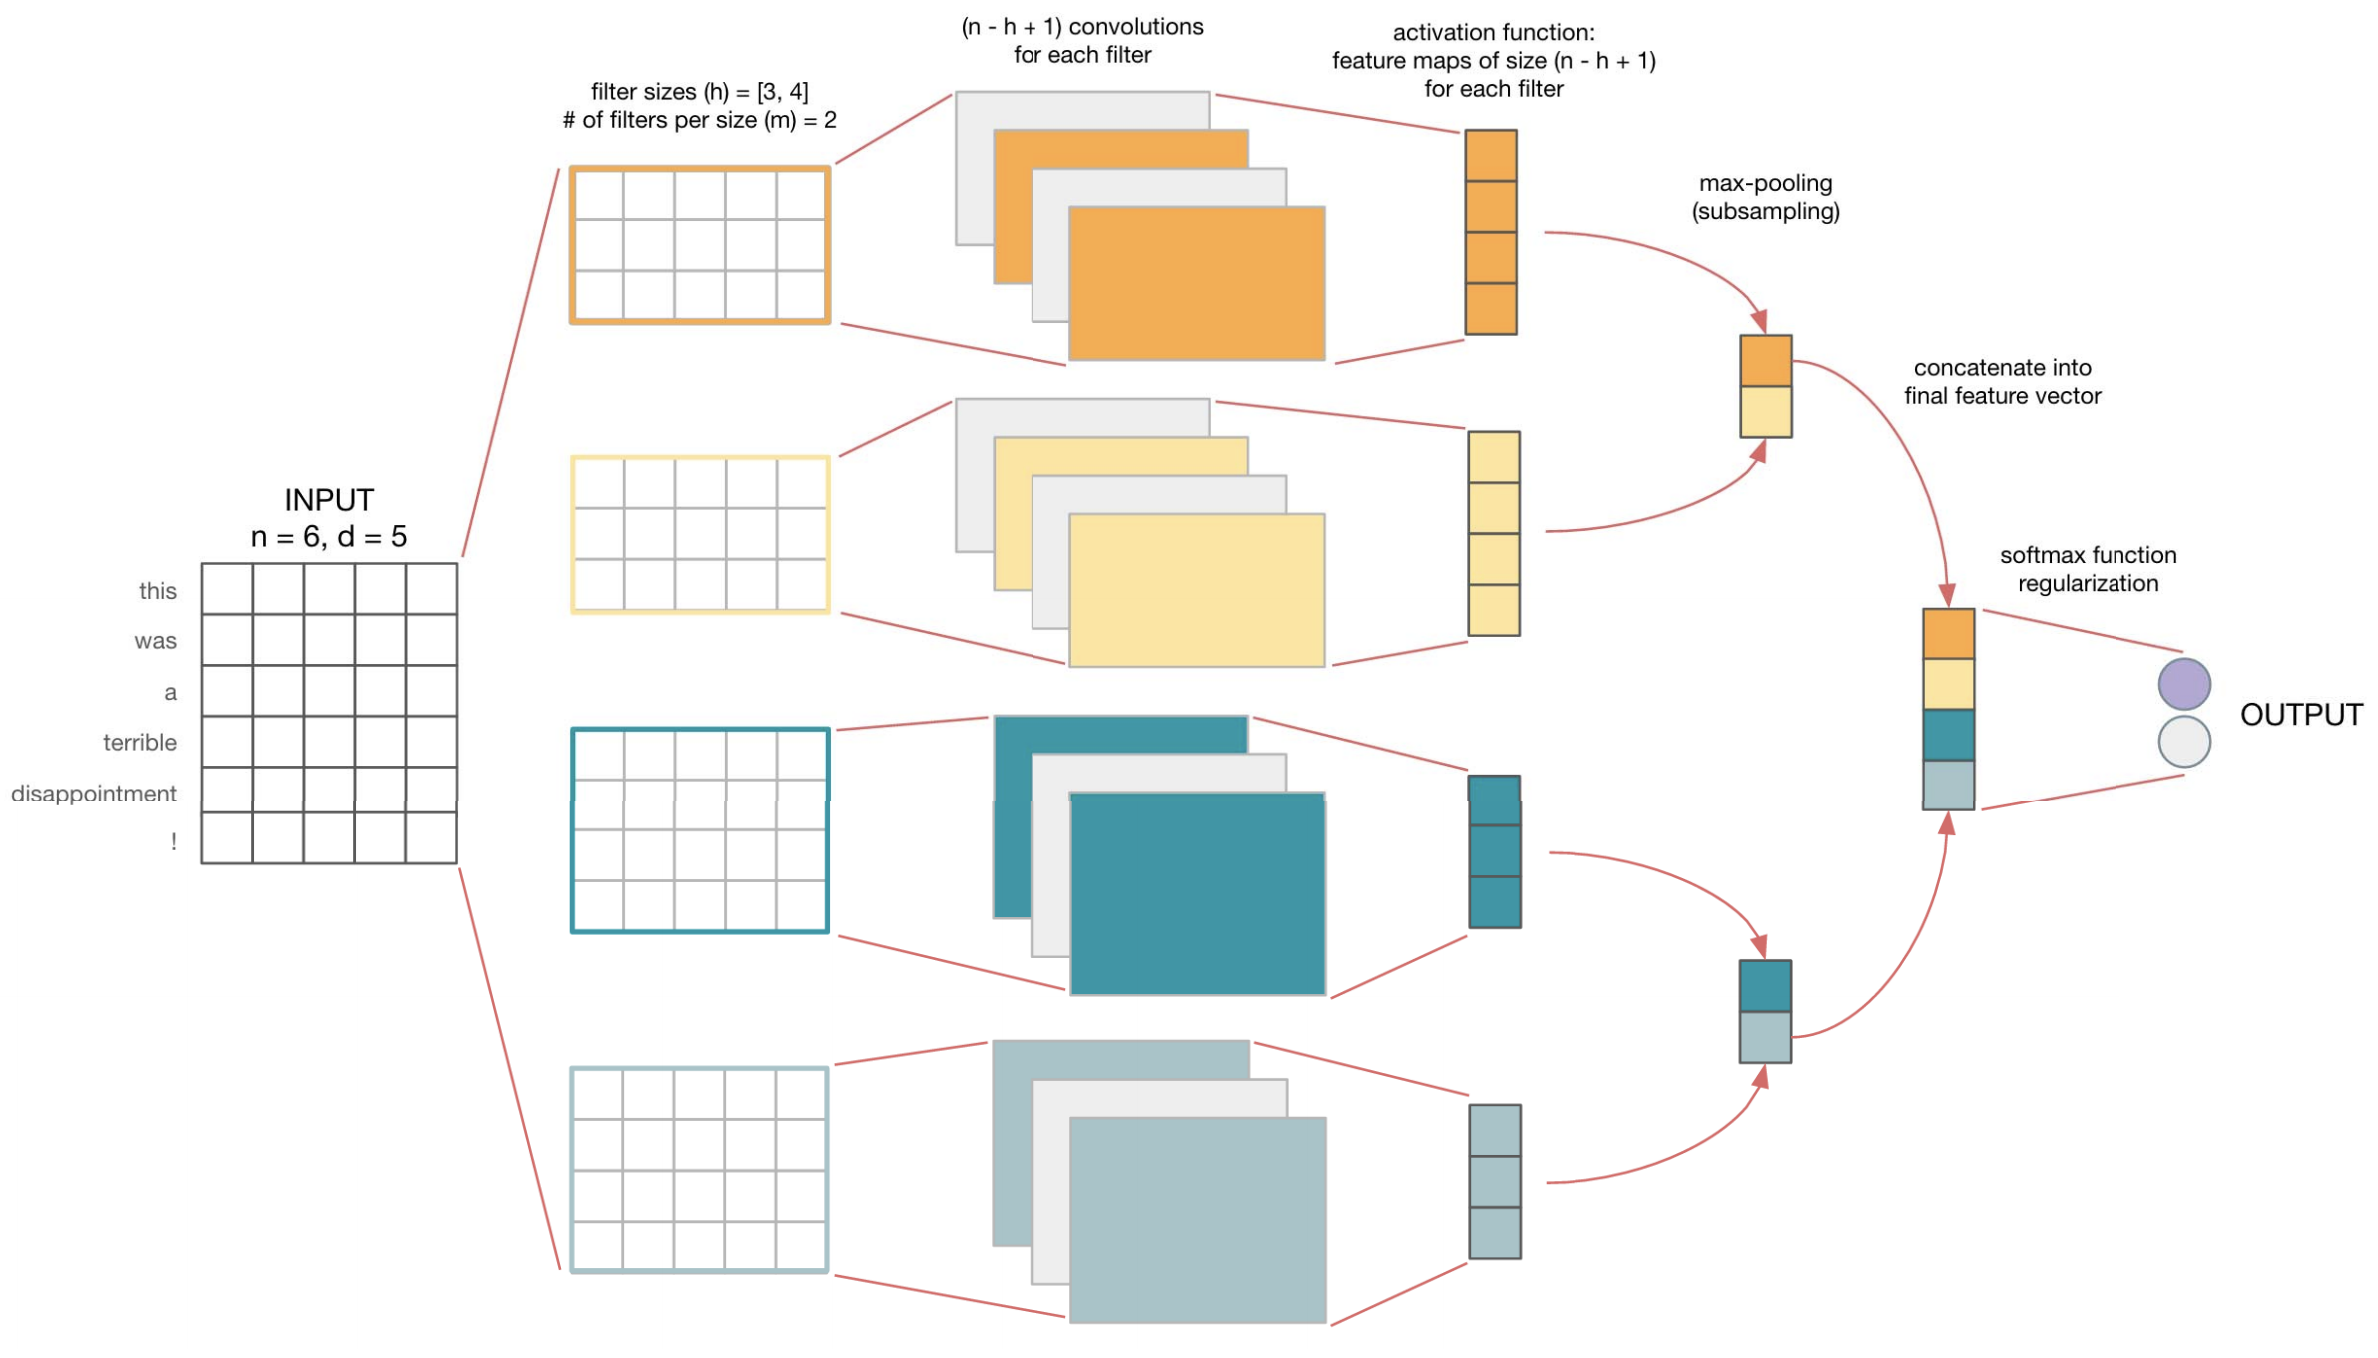
\includegraphics[width=450px]{img/CNN Word2vect.png}
    \caption{Esquema de la red utilizada}
    \end{figure}

\vspace{3mm}

La arquitectura propuesta muestra un conjunto de convoluciones que hace posible aplicar numerosos filtros de varios tamaños de forma que se representan así los distintos n-gramas de cualquier frase. Posteriormente se aplican mapas de características y se acaba con una clasificación binaria de los requisitos.

\vspace{3mm}

Los resultados obtenidos por los autores demuestran que la inclusión de \textit{embeddings} hace que se mejore la precisión (\textit{precision}) sin sacrificar la sensibilidad (\textit{recall}), obteniendo un F1-Score del 7\%. \textbf{Por todo ello resulta muy interesante aplicar técnicas similares a las propuestas por los autores a la clasificación de géneros de libros propuesta en este documento}.

\newpage

\section{Conjunto de datos}
    En esta sección se describe el \textbf{conjunto de datos} utilizado en su forma original, así como todos los cambios que se hacen como parte del \textbf{preprocesado} junto con las razones que han llevado a su realización.

    \subsection{Estructura original}
    El conjunto de datos ha sido obtenido de \textbf{Kaggle} [https://www.kaggle.com/meetnaren/goodreads-best-books/activity], y dispone de un total de \textbf{54283 libros y 12 columna} con información sobre ellos. En la Figura X se puede apreciar visualmente la forma de las instancias de este conjunto de datos.

    \vspace{3mm}

    \begin{figure}[!h]
        \centering
        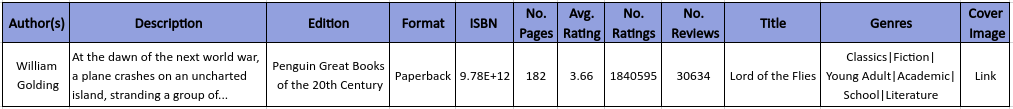
\includegraphics[width=500px]{img/instancia_dataset_original.png}
        \caption{Instancia del conjunto de datos original}
    \end{figure}

    \vspace{3mm}

    A continuación se explica el \textbf{contenido} de cada columna en más detalle:

    \begin{itemize}
        \item \textbf{Author(s):} Cadena de caracteres que indica el o los autores del libro. En caso de ser más de uno, cada autor aparece separado por '$\mid$'.
        \item \textbf{Description:} Cadena de caracteres que indica el resumen o descripción del libro.
        \item \textbf{Edition:} Cadena de caracteres que indica la edición del libro.
        \item \textbf{Format:} Cadena de caracteres que indica el formato del libro, como por ejemplo \textit{handcover} o \textit{paperback}.
        \item \textbf{ISBN:} Valor numérico que indica el ISBN del libro. Debido a que se utiliza notación científica para su representación, no se puede leer ni usar correctamente, pues faltan números.
        \item \textbf{No. Pages:} Valor numérico que indica el número de páginas que tiene el libro.
        \item \textbf{Avg. Rating:} Valor numérico que indica la valoración media que los usuarios han dado al libro.
        \item \textbf{No. Ratings:}  Valor numérico que indica la cantidad de valoraciones de usuario que ha recibido el libro.
        \item \textbf{No. Reviews:} Valor numérico que indica la cantidad de críticas que ha recibido el libro.
        \item \textbf{Title:} Cadena de caracteres que indica el título del libro.
        \item \textbf{Genres:} Cadena de caracteres que indica los géneros a los que pertenece el libro. Los diferentes géneros aparecen separados por '$\mid$'.
        \item \textbf{Cover Image:} Imagen que muestra la portada del libro. Se indica un enlace que lleva hasta dicha imagen, aunque por motivos de espacio no se ha incluido en la figura de arriba.
    \end{itemize}

    \vspace{3mm}

    En un primer momento se consideró usar el conjunto de datos \textbf{CMU Book Summary Dataset} [https://www.cs.cmu.edu/~dbamman/booksummaries.html], pero la manera en la que estaban dispuestos los géneros, así como el resto de atributos, daba lugar a un \textbf{procesado más complejo} para obtener sus valores.

    \vspace{1mm}

    Además, se consideró que los géneros que se utilizaban no eran muy acertados, como por ejemplo \textit{Speculative fiction} o \textit{Postmodernism}. Posteriormente se encontró el conjunto de datos que se ha descrito arriba, el cual tiene muchas más instancias (54,283 frente a 16,559), proporciona mucha más información (tiene más atributos) y, lo más importante, es mucho más sencillo obtener los valores de sus instancias.

    \subsection{Preprocesado}
        En toda tarea de Minería de Texto existe algún tipo de \textbf{preprocesado}, ya sea obtener sólo los valores que se necesiten, eliminar instancias con errores, vectorizar el texto, etc. Esta vez no va a ser diferente, e incluso se puede afirmar que ha sido una \textbf{parte importante del trabajo}, y que ha ocupado una cantidad considerable de tiempo. A continuación se detallan todas las \textbf{modificaciones} que se han llevado a cabo:

        \begin{itemize}
            \item \textbf{Selección de las columnas útiles:} De las 12 columnas que tiene el conjunto de datos seleccionado, solo son necesarias dos, \textit{description} y \textit{genres}, que contenían, respectivamente, el resumen o descripción del libro y los géneros que se le atribuyen. Por ello, solo solo se mantendrán dichas columnas eliminando el resto.
            \item \textbf{Eliminación de instancias con descripciones en un lenguaje diferente al ingles:} Los resúmenes del conjunto de datos se encuentran escritos no solo en inglés, si no también en árabe, italiano, chino, coreano, japonés, portugués...Se ha decidido por razones evidentes, mantener solo aquellos libros cuyos resúmenes estén en ingles. Para la detección del idioma se ha utilizado la librería \textit{\textbf{langdetect}} [https://pypi.org/project/langdetect/] de \textit{Python}, y aquellas instancias donde se detectaba un idioma diferente al inglés se han borrado. Gracias a la gran cantidad de instancias que hay, la eliminación de las instancias no afecta de manera significativa.
            \item \textbf{Corrección de formatos incorrectos:} Algunos de los resúmenes del conjunto de datos contenían errores de formato como saltos de línea (de diferentes tipos), tabulaciones o espacios en medio de los resúmenes, así que se sustituyeron por un único espacio en blanco.
            \item \textbf{Eliminación de caracteres no útiles:} Se han eliminado de los resúmenes del conjunto de datos caracteres que no proporcionaban ningún tipo de información, como comillas, guiones, corchetes, paréntesis, puntos, exclamaciones, interrogaciones, etc.
            \item \textbf{Eliminación de términos no útiles:} Se han eliminado de los resúmenes del conjunto de datos términos que no proporcionaban ningún tipo de información útil. Para ello se ha utilizado una lista de \textit{\textbf{stopwords}}, reutilizada de la segunda práctica de la asignatura, pero a la cual se han añadido términos que se han ido encontrado al realizar pruebas. Evidentemente, no se han incluido todos los términos sin información útil posibles, pero dada la gran cantidad de términos que puede haber, creemos que la cantidad de \textit{\textbf{stopwords}} obtenida es suficiente.
            \item \textbf{Cambios requeridos por la aproximación usada:} La aproximación que se utilizada en este trabajo requiere que los resúmenes esté en minúsculas. Al contrario que ocurría en la segunda práctica, no es necesario dividir los resúmenes en términos, por lo que no se utilizara la cadena de caracteres que contiene el resumen de manera directa.
            \item \textbf{Eliminación de géneros no útiles:} Después de analizar un poco más a fondo los diferentes géneros que se usan, se ha observado la falta de un criterio claro para elegir que géneros usar, dando lugar a géneros de países, como \textit{spain}, al mismo tiempo que el género \textit{spanish literature}. También se encontraron géneros muy concretos y sin mucho sentido, como \textit{Amazon} o \textit{Apple}. Esto llevó a que fuera necesario revisar manualmente todos los géneros, los cuales eran en torno a 850, y eliminar aquello que se consideraron no útiles. Al finalizar esta revisión quedaron 625 géneros.
        \end{itemize}

    \vspace{3mm}

    Una vez aplicado todo esto, los datos ya están preparados para su uso. Sin embargo, queda una última cosa. La cadena de caracteres que contiene los géneros se separara según el caracter '$|$' en los diferentes géneros para su posterior uso. Como en este trabajo se va explorar una clasificación \textbf{multi-clase} con el primer género, y una clasificación \textit{\textbf{multi-label}} con todos los géneros, para la primera solo se utilizará el primer género, y para la segunda se usarán todos.

\newpage

\section{Conceptos teóricos}
A la hora de elegir un método de Minería de Texto se consideran diversas opciones tales como utilizar la herramienta \textit{Weka} de la \textit{Universidad de Waitako}. Sin embargo, dado que esta herramienta ya ha sido utilizada a lo largo de la asignatura y, además, presenta ciertas limitaciones en cuanto a la flexibilidad y capacidad de toma de decisiones de diseño en los modelos, se decide aplicar \textbf{Word Embedding} en Redes de Neuronas con la \textbf{biblioteca de código abierto \textit{Tensorflow}}. De esta manera se usa un método diferente al usado en clase, lo cual permite experimentar y aprender tecnologías nuevas.

\vspace{3mm}

No obstante, antes de iniciar la codificación del modelo, dado que se trata de una técnica nueva, es necesario tener claros los conceptos teóricos involucrados. Una Red Neuronal únicamente procesa números, lo que implica que es necesario realizar una transformación. Representar las palabras como vectores es importante, ya que los modelos de IA no ‘entienden’ las palabras, y no pueden realizar cálculos ni aprendizaje sobre ellas. Por este motivo, es necesario realizar una \textbf{vectorización}, que no es más que transformar estas palabras en números, agrupados en forma de vector. A continuación se exponen las diferentes técnicas de vectorización consideradas.

\subsection{Codificación con valor único}
Una primera aproximación podría ser asignar un único número a cada una de las palabras consideradas en la vectorización. Por ejemplo, con la frase 'hace un espléndido día' se obtiene un vector como el que sigue:

      \begin{table}[h]
        \centering
        \begin{tabular}{|c|c|}
        \hline
        \rowcolor[HTML]{DAE8FC}
        \textbf{Palabra} & \textbf{Valor} \\ \hline
        hace                    & 1   \\ \hline
        un                     & 2   \\ \hline
        espléndido                     & 3  \\ \hline
        día                       & 4   \\ \hline
        \end{tabular}
        \caption{Codificación con un único valor}
            \label{fig:graf_exp1}
    \end{table}

Este enfoque presenta una serie de consideraciones importantes:
\begin{itemize}
\item El valor de cada palabra se decide de manera arbitraria.
\item No se obtiene una representación fiel de la distancia entre palabras, lo cual es un hecho que es importante en el desarrollo de esta práctica.
\end{itemize}

Por ello, se descarta el enfoque aquí propuesto por no ser eficiente en la tarea a realizar.

\subsection{One-hot encoding}
La codificación \textit{one-hot} consiste en convertir cada palabra en un vector con tantas posiciones como palabras se tengan, con un 1 en la posición que se corresponda a la palabra considerada y un 0 en caso contrario.


\vspace{2mm}

A continuación se muestra un ejemplo de la codificación con el pequeño set de palabras utilizado en la sección anterior.

\newpage

  \begin{table}[!h]
        \centering
        \begin{tabular}{|c|c|c|c|c|}
        \hline
        \textbf{} &\textbf{hace} & \textbf{un} & \textbf{espléndido} & \textbf{día}  \\ \hline
        \textbf{hace}                     & 1 & 0 & 0 & 0\\ \hline
        \textbf{un}                       & 0 & 1 & 0 & 0\\ \hline
        \textbf{espléndido}               & 0 & 0 & 1 & 0\\ \hline
        \textbf{día}                      & 0 & 0 & 0 & 1\\ \hline
        \end{tabular}
        \caption{One-hot encoding}
            \label{fig:graf_exp1}
    \end{table}

\vspace{2mm}

El principal problema de esta técnica de vectorización es que la distancia entre las palabras es la misma, lo cual impide de nuevo disponer de una representación realista de este hecho esencial en el enfoque que se propone.

\subsection{Embedding}

Está técnica sirve para representar aquellas \textbf{palabras que son semánticamente parecidas con una codificación similar}. Lo que hace esta técnica tan atractiva es que no es necesario especificar esta similitud de forma manual.

\vspace{2mm}

Un \textit{embedding} es un vector denso de números reales, donde su longitud viene determinada por parámetro. En lugar de determinar los pesos a mano, se tratan como \textbf{parámetros que pueden ser entrenados}, como si de pesos de Redes de Neuronas densas se trataran. Por eso mismo, esta técnica funciona especialmente bien con las Redes de Neuronas, que incorpora la modificación de estos pesos a la fase de entrenamiento de la red.

\vspace{2mm}

La dimensionalidad del \textit{embedding} debe ser proporcional a la cantidad de datos disponibles, ya que cuanto más grande sea el vector, más detalles podrá obtener de cada palabra, pero requiere de más datos para ser entrenado. La siguiente tabla muestra un ejemplo de la codificación con el pequeño conjunto de palabras utilizado en la sección anterior.

  \begin{table}[h]
        \centering
        \begin{tabular}{|c|c|c|}
        \hline
        \textbf{hace}                     & 2.32 & 7.35 \\ \hline
        \textbf{un}                       & 0.89 & 4.23 \\ \hline
        \textbf{espléndido}               & 0.75 & 8.65 \\ \hline
        \textbf{día}                      & 2.65 & 3.00 \\ \hline
        \end{tabular}
        \caption{Embedding}
            \label{fig:graf_exp1}
    \end{table}

Por lo tanto, esta técnica resulta de gran utilidad a la hora de conseguir representar la distancia semántica entre las palabras que forman un texto. Siendo este hecho fundamental para la tarea propuesta \textbf{se decide apostar por esta codificación para construir el modelo de \textit{Text Mining}}.

\newpage

\section{Clasificación}

Normalmente un libro se encuadra en más de un género literario, por ello, de manera inicial se decide enfocar el problema en la clasificación de un solo género para posteriormente, poder realizar una ampliación del algoritmo que prediga todos los géneros posibles de un escrito.

\vspace{2mm}

Dado que la técnica que se desea utilizar es prácticamente exclusiva para los modelos de Redes de Neuronas, este es el acercamiento que se decide implementar.

\subsection{Arquitectura del modelo}

Una vez se cargan los datos preprocesados se realiza una aleatorización de los mismos para evitar posibles sesgos, se vectorizan las salidas y se dividen los datos en conjunto de  entrenamiento (70\%) y en conjunto de test (30\%). Los modelos considerados siguen todos la misma estructura de Red de Neuronas:

\begin{itemize}
\item \textbf{Capa de vectorización del texto}: Transforma cadenas de caracteres a índices de vocabulario, el vocabulario se crea a partir de la frecuencia de valores individuales. Se modifican los siguientes parámetros:
\begin{itemize}
\item \textbf{Número máximo de tokens}: Representa el tamaño del vocabulario a usar.
\item \textbf{Longitud de la secuencia de salida}: número de índices de palabras que se pasa a la capa siguiente.
\end{itemize}

\item \textbf{Capa de \textit{embedding}}: A partir del vocabulario busca el vector de \textit{embedding} para cada índice de palabras. Estos vectores se aprenden según el modelo se entrena.

\item \textbf{Capa de agrupación promedio global}: Devuelve un vector de salida de longitud fija para cada ejemplo haciendo la media sobre la dimensión de la secuencia. Se utiliza para permitir a la red usar los datos del \textit{embedding}.

\item \textbf{Capa densa}: Neuronas completamente conectadas. Según el modelo puede tener una o varias capas y el número de neuronas puede variar por capas.

\item \textbf{Capa de salida}: Capa densa que tiene tantas neuronas como géneros distintos haya.

\end{itemize}

De forma gráfica se puede presentar la estructura como se muestra en la Figura X.

  \begin{figure}[!h]
    \centering
    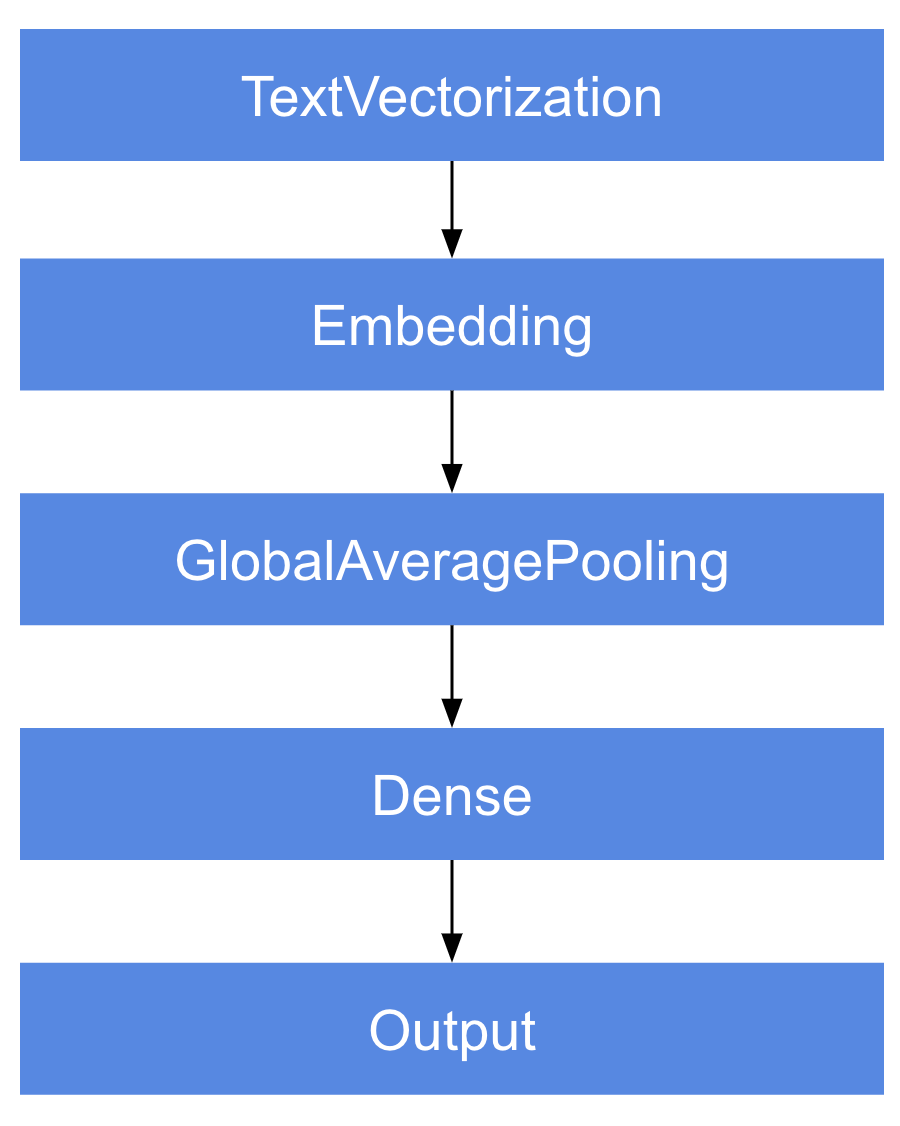
\includegraphics[width=150px]{img/Arquitectura.png}
    \caption{Arquitectura del modelo}
    \end{figure}


\newpage


\subsection{Clasificación de 1 género}

La idea de usar un sólo género a la hora de clasificar un libro es útil si este género es el principal del mismo, sin embargo, el \textit{conjunto de datos} original no hace una diferenciación sobre esto y establece todos los géneros de un libro con la misma importancia. Por ello, se ha decidido guardar el primer género de cada libro, aunque esto \textbf{podría suponer un sesgo }sobre el modelo, el cual se debe tener en cuenta.

\vspace{2mm}

Por ejemplo, si un libro pertenece a los géneros Ciencia ficción, Aventura y Fantasía, al entrenar únicamente con el primer género puede que la salida la red lo clasifique como Fantasía y lo trate como un error al desconocer que también pertenece a este género. Por ello, es de suma importancia realizar la ampliación multi-género.

\vspace{3mm}

Al realizar las transformaciones oportunas seleccionando el primer género \textbf{se obtienen un total de 194 géneros diferentes}. Se trata por lo tanto de un problema de clasificación multi-clase ya que se tienen 194 clases y cada instancia tiene una sola etiqueta.

\vspace{3mm}

Para poder ser utilizadas por la red, las salidas se vectorizan usando \textit{one-hot encoding} para representar a estas clases, donde cada posición es un género distinto. Un 0 significa que no pertenece a ese género y un 1 que sí pertenece. Por lo tanto, la forma que tiene el vector de una salida cualquiera es: [0, 0, …, 0, 1, …, 0]. El cual tiene tamaño 194 y un sólo 1.

\vspace{3mm}

Otro aspecto importante que hay que tener en cuenta al tratarse de un problema multi-clase es la función de coste. Se usa \textbf{entropía cruzada categórica} (\textit{Categorical Cross-Entropy}) porque se desea entrenar a la red para sacar como salida la probabilidad para todas las clases sobre cada uno de los ejemplos. Esta función de coste es la más utilizada en problemas de clasificación multi-clase, e indica el porcentaje de veces que el modelo otorga el valor más alto de creencia a la clase acertada.

\vspace{3mm}

La Figura X muestra un ejemplo de la codificación \textit{one-hot} en la vectorización de los géneros de la novela '1984'.

  \begin{figure}[!h]
    \centering
    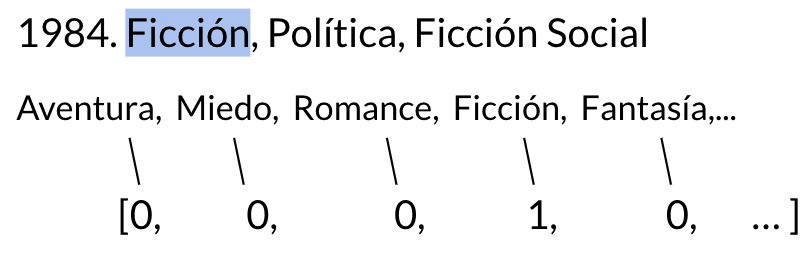
\includegraphics[width=250px]{img/1984_Genres.png}
    \caption{One-hot encoding de 1 género}
    \end{figure}

\newpage

\subsection{Clasificación multi-género}
Por el sesgo comentado en el apartado anterior al elegir solo el primer género, se ha decidido implementar también la clasificación de todos los géneros. Sin embargo, esto \textbf{aumenta significativamente la dificultad} del problema, pues para un mismo texto hay diferentes géneros, además de que no todos los libros pertenecen a la misma cantidad de géneros.

\vspace{3mm}

Al separar todos géneros se obtienen \textbf{625 géneros diferentes}, que es una cantidad tres veces mayor que en el problema de un único género. Se trata de un problema \textit{multi-label}, ya que cada instancia puede pertenecer a una o más etiquetas.

\vspace{3mm}

La vectorización de la salida ocurre de la misma manera que en caso de un único género, salvo que ahora este vector tendrá una longitud de 625, y tendrá tantos unos como cantidad de géneros a los que el libro pertenezca. En la Figura X se muestra la codificación \textit{one-hot} en la vectorización de la salida para un libro que pertenece a los géneros: ficción, aventura y fantasía.

  \begin{figure}[!h]
    \centering
    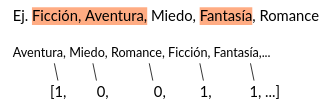
\includegraphics[width=250px]{img/ej_one_hot_multi.png}
    \caption{One-hot encoding multi-género}
    \end{figure}

Por último, esta vez como función de coste se utiliza \textbf{entropía cruzada binaria} (Binary Cross-Entropy), debido a que funciona de manera independiente para cada clase, o en este caso, género.

\section{Experimentación y análisis}

Con el objetivo de obtener los mejores resultados, es necesario realizar una experimentación que modifique los distintos hiper-parámetros del modelo. Dado que la tecnología usada está ligada con las Redes de Neuronas, se ha probado exclusivamente con este tipo de modelos. Los parámetros que se han decidido modificar son:

\begin{itemize}
  \item \textbf{Batch Size}: Hace referencia al tamaño de los lotes, es decir, cada cuantos individuos se actualizan los pesos de la red. Un tamaño mayor lleva a un menor tiempo de ejecución, y menos especificidad sobre los ejemplos.
  \item \textbf{N Grams}: Número máximo de palabras que puede tener un \textit{token}.
  \item \textbf{Sequence Length}: Número de índices de palabras que recibe la capa de \textit{embedding}.
  \item \textbf{Vocab Size}: Tamaño total del vocabulario a usar. El vocabulario está compuesto de las palabras más comunes en los textos.
  \item \textbf{Embedding Dimension}: Tamaño de los vectores de \textit{embedding}.
  \item \textbf{Topology}: Topología de las capas densas de la red. En caso de que incluyan una capa de \textit{dropout}, se representa con una \textbf{D} acompañado de su valor.
\end{itemize}

Para los resultados obtenidos, el número de ciclos se calcula para que tenga el valor óptimo para cada uno de los experimentos para evitar el sobre aprendizaje.

\vspace{2mm}

La métrica que se decide usar es \textit{Categorical Accuracy}, dado que se tiene más de una clase sobre la que clasificar.


\subsection{Modelo 1 género}

Este primer acercamiento se hace exclusivamente con el primer género de cada libro. A través de este acercamiento se tienen \textbf{194 clases}, por tanto, la última capa del modelo posee \textbf{194 neuronas}.

\vspace{2mm}

Los experimentos que se han realizado para este acercamiento se han ido creando progresivamente según se buscaba mejorar los resultados. Se van modificando los hiper-parámetros con el fin de conseguir el mayor \textit{accuracy} en test.

\vspace{1mm}

A continuación se muestra una tabla que resume esta experimentación y los resultados obtenidos, Figura X:

\newpage

\begin{figure}[!h]
    \centering
    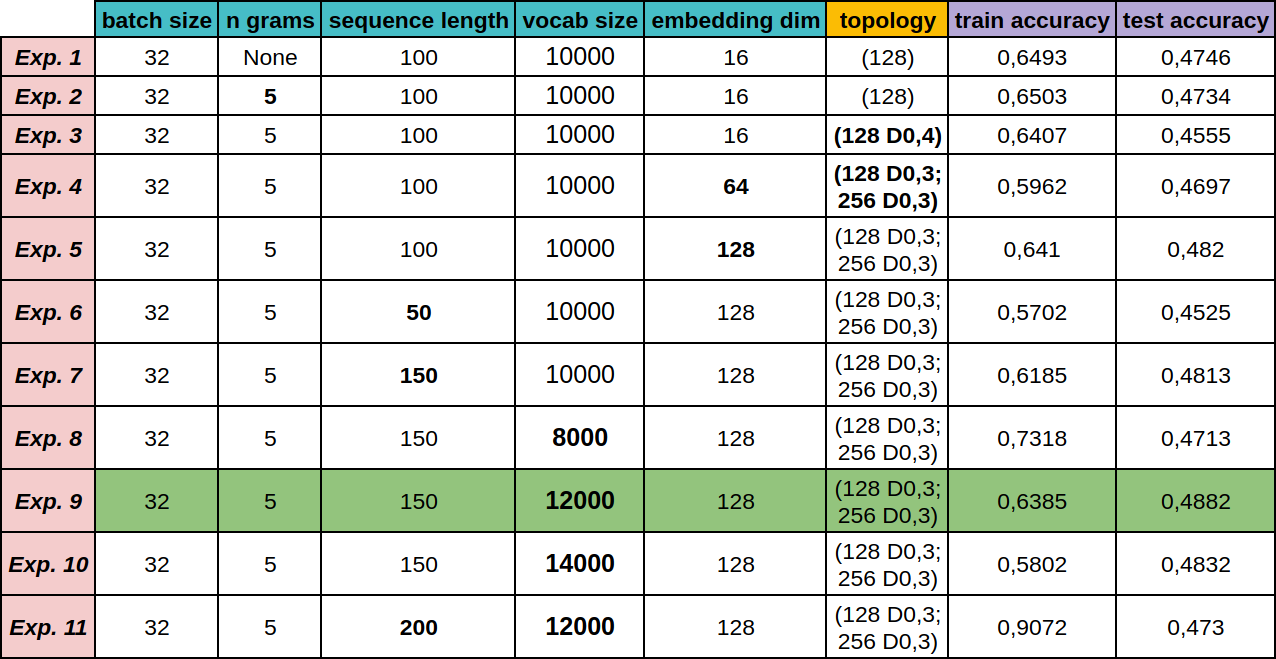
\includegraphics[width=500px]{img/one.png}
    \caption{Resumen experimentación y resultados del modelo 1 género}
\end{figure}

Como se puede apreciar en la tabla de la Figura X, los resultados son bastante aceptables, con valores de \textit{accuracy} en test que se encuentran entre el \textbf{47\%} y \textbf{48\%}, siendo el \textbf{Exp. 9} el que mejores resultados genera con un \textbf{48,82\%}. Aun así, se puede ver que los resultados obtenidos no varían demasiado según los hiper-parámetros. Los análisis que se pueden realizar sobre estos hiper-parámetros son:

\begin{itemize}
  \item Aumentar la complejidad de la red genera mejores resultados.
  \item Si se intenta disminuir el \textit{batch size}, el tiempo de computo crece exponencialmente, así que no se ha modificado. Se ha decidido no aumentarlo por encima de 32 porque, como dijo Yann LeCun, padre fundador de las redes convolucionales, \textit{'Training with large minibatches is bad for your health. More importantly, it's bad for your test error. Friends dont let friends use minibatches larger than 32'}(https://twitter.com/ylecun/status/989610208497360896?lang=es).
  \item Usar \textit{ngrams} es útil. Se decide usar tamaño 5, aunque en la exploración del vocabulario, el tamaño máximo de \textit{ngram} es 4, y la gran mayoría de ellos mantiene el tamaño 1. Se usa para permitir \textit{ngrams} de cualquier tamaño.
  \item Se prueban diferentes valores de \textit{sequence length}, y los mejores resultados se encuentran con valores de 150.
  \item El tamaño del vocabulario que se ha probado que mejor funciona es 12000.
  \item Aumentar el tamaño del \textit{embedding} mejora los resultados, pero también aumenta considerablemente el tiempo de ejecución. Por eso no se aumenta por encima de 128.
\end{itemize}

  A pesar de que los resultados son mejorables, se considera un buen acercamiento a este problema, asumiendo que es una simplificación del problema real. También hay que tener en cuenta que este problema tiene un gran sesgo que puede deberse a que tan solo se coge un único género, por lo que la red puede que esté clasificando un género del libro realmente, pero no es conocido por el modelo, y por tanto lo trata como un error.

  \vspace{2mm}

  Por ejemplo, si un libro pertenece a \textbf{Aventura} y \textbf{Ciencia ficción}, y el modelo lo clasifica como \textbf{Ciencia ficción}, se considerará un error.



\subsection{Modelo multi-género}

La experimentación que se lleva a cabo para este segundo acercamiento se hace con todos los géneros que puede llegar a tener un libro. Con esto se pretende ampliar el problema, e intentar determinar todos los posibles géneros de un libro, acercándose más a un problema real. Pero hay que tener en cuenta que se tienen \textbf{625 clases} por lo que la última capa del modelo tiene \textbf{625 neuronas}, lo que aumenta la complejidad del acercamiento. Además como se trata de un problema multi-etiqueta, su dificultad es todavía mayor.

\vspace{2mm}

El proceso de creación de los experimentos se basa en ir modificando la configuración de los hiper-parámetros ligeramente para encontrar aquella con la que se obtienen mejores resultados. Se van subiendo o bajando estos valores para intentar alcanzar un \textit{accuracy} en test lo más alto posible.

\vspace{1mm}

En la Figura X se muestra una tabla resumen de todos los experimentos realizados junto con sus resultados:


\begin{figure}[!h]
    \centering
    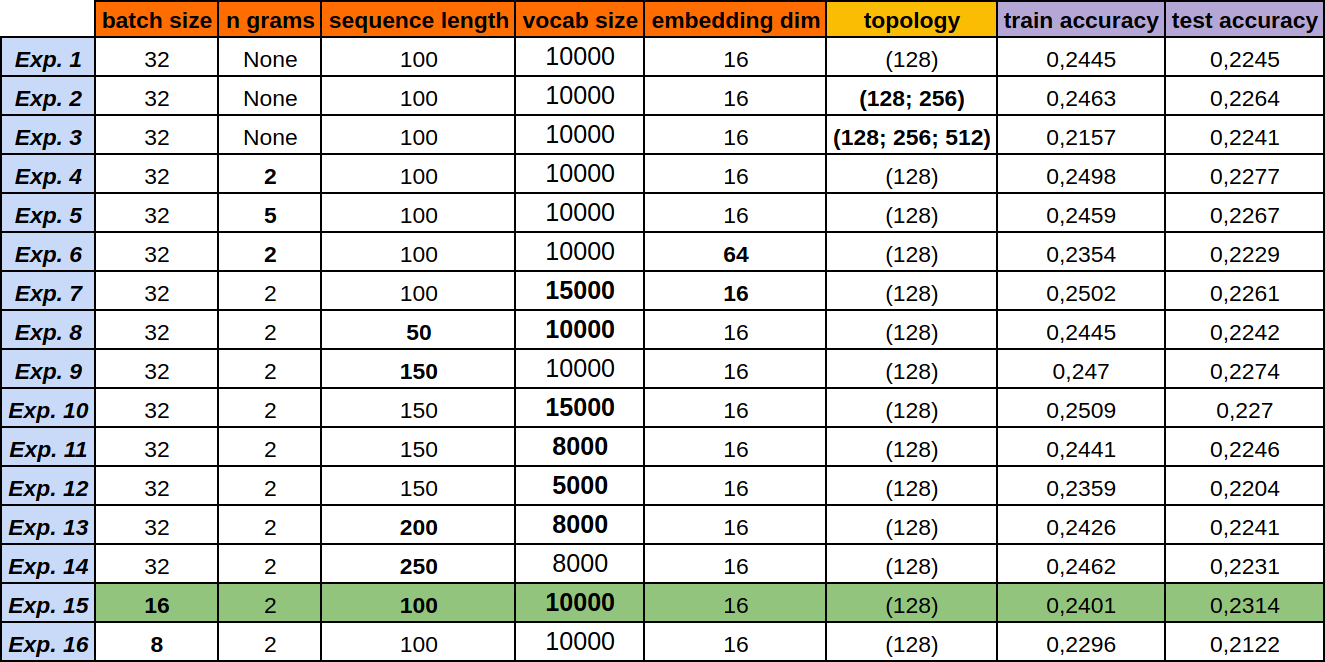
\includegraphics[width=500px]{img/multi.png}
    \caption{Resumen experimentación y resultados del modelo multi-género}
\end{figure}

Las conclusiones a las que se llegan son:

\begin{itemize}
  \item Aumentar la complejidad de la topología no mejora los resultados.
  \item Utilizar \textit{2 grams} es positivo y genera mejores resultados, aunque inspeccionando el vocabulario, se comprueba que no hay muchos \textit{ngrams} que sean de tamaño 2.
  \item El tamaño de vocabulario de 10000 palabras es el más adecuado en este caso.
  \item El tamaño del vector de \textit{embedding} de 16 posiciones es el que mejor funciona.
  \item El número de índices que recibe la capa de \textit{embedding} se prueba con distintos valores pero se obtienen mejores resultados con 100.
  \item El \textit{batch size} se modifica en los últimos experimentos consiguiendo una mejora de resultados con un tamaño de 16.
\end{itemize}


Por tanto se concluye con que el mejor experimento es el \textbf{Exp. 15}, con un \textit{accuracy} en test de \textbf{23,14\%}. Este valor no es especialmente alto pero, dada la complejidad del problema, se puede considerar como un éxito.





\subsection{Caso de uso}







\section{Conclusiones}
Respecto a la asignatura en sí, este trabajo ha servido para observar en primera persona la realización de un \textbf{tarea \textit{real}}, donde ha habido que buscar diversos conjuntos de datos, analizarlos, y elegir el que mejor se adecuaba a las necesidades del problema. Después, ha sido necesario un \textbf{preprocesado importante}, donde se han encontrado problemas con una complejidad mayor que los que aparecen en el resto de prácticas de la asignatura (y en otras en general). 

\vspace{3mm}

Por último se comprende que \textbf{es posible no obtener datos muy buenos}, pues, de nuevo, es un problema complicado de resolver.  Todo lo comentado muestra lo diferente que son los problemas del \textbf{mundo académico} a los del \textbf{mundo real} o problemas que no están tan acotados.

\vspace{3mm}

Poniendo la atención sobre la rama de la Inteligencia Artificial utilizada, la \textbf{minería de datos}, comentar que es un ámbito, no solo \textbf{complejo}, si no además muy \textbf{variado}. Se ha optado por la aproximación realizada por el hecho de incluir variedad en la aproximaciones utilizadas en la asignatura, así como para usar una técnica que sea mas personalizable que las vistas en clase. 

\vspace{3mm}

Sin embargo, esto no quiere decir que algunas técnicas mas clásicas o simples funcionarán peor. Si el alcance de este trabajo fuera mayor y se dispusiera de mas tiempo, sería casi imperativo \textbf{probar otras técnicas} (vistas y no vistas en clase) y realizar una comparación entre ellas de manera exhaustiva.

\clearpage

\bibliographystyle{ieeetr}
\bibliography{bibliografia.bib}


\end{document}
